% !TEX root = ../OT4ML.tex

%%%%%%%%%%%%%%%%%%%%%%%%%%%%%%%%%%%%%%%%%%%%%%%%%%%%%%%%%%%%%%%%%%%%%%%%%%%
%%%%%%%%%%%%%%%%%%%%%%%%%%%%%%%%%%%%%%%%%%%%%%%%%%%%%%%%%%%%%%%%%%%%%%%%%%%
%%%%%%%%%%%%%%%%%%%%%%%%%%%%%%%%%%%%%%%%%%%%%%%%%%%%%%%%%%%%%%%%%%%%%%%%%%%
\chapter{Dual Problem}
\index{dual!problem}% strictindex
\label{sec-dual}

Duality turns the transport problem into a search for potentials rather than couplings. This chapter explains why potentials certify optimality, how $c$-transforms regularize them, and why the quadratic case reveals convex analysis behind Brenier maps. Linear-programming duality gives the discrete picture~\cite{bertsimas1997introduction}, while the continuous form is one of the central theorems of OT~\cite{Villani03,SantambrogioBook}.
\index{Brenier!map}% strictindex
\index{c-transform}% strictindex

%%%%%%%%%%%%%%%%%%%%%%%%%%%%%%%%%%%%%%%%%%%%%%%%%%%%%%%%%%%%%%%%%%%%%%%%%%%
\section{Discrete dual}
\label{sec-discrete-dual}


The discrete dual gives finite-dimensional certificates of optimality. Its complementary slackness conditions identify where an optimal coupling can put mass.
\index{optimal coupling}% strictindex
\index{complementary slackness}% strictindex

The Kantorovich problem~\eqref{eq-kanto-discr} is a linear program so that one can equivalently compute its value by solving a dual linear program.
\index{Kantorovich!problem}% strictindex

% a constrained convex minimization problem, and as such, it can be naturally paired with a so-called dual problem, which is a constrained concave maximization problem. The following fundamental proposition, which is a special case of Fenchel-Rockafellar duality theory, explains the relationship between the primal and dual problems.

\begin{defn}[Admissible potentials]\label{def-admissible-potentials}
\index{admissible potential}% strictindex
\index{dual!potential}% strictindex
	For a discrete problem with marginal sizes $n,m$ and cost matrix $\C\in\RR^{n\times m}$, a pair $(\fD,\gD)\in\RR^n\times\RR^m$ is admissible if it lies below the cost:
	\eql{\label{eq-feasible-potential}
		\PotentialsD(\C) \eqdef \enscond{
			(\fD,\gD) \in \RR^n \times \RR^m
		}{ \foralls (i,j) \in \range{n} \times \range{m}, \fD_i+\gD_j \leq \C_{i,j} }.
	}
	Equivalently, $\fD\oplus\gD\leq\C$ entrywise. In particular, the feasible set depends on the cost matrix, not on the marginal weights.
\end{defn}
The two vectors play the role of source and target prices; admissibility means that no transported pair is priced above its travel cost.

\begin{prop}[Discrete Kantorovich duality]\label{prop-duality-discr}
\index{Kantorovich!duality}% strictindex
One has
\eql{\label{eq-dual}
	\MKD_\C(\a,\b) =
	\umax{(\fD,\gD) \in \PotentialsD(\C)} \dotp{\fD}{\a} + \dotp{\gD}{\b}.
}
\end{prop}

\begin{proof}
For completeness, introduce multipliers $(\fD,\gD)$ for the two marginal constraints. The Lagrangian is
\index{dual!problem}% strictindex
\eql{\label{eq-mk-lagr}
	\mathcal L(\P,\fD,\gD)
	=\dotp{\C}{\P}+\dotp{\a-\P\ones_m}{\fD}
	+\dotp{\b-\P^\top\ones_n}{\gD}.
}
For fixed potentials, the dual function is
\[
	\inf_{\P\geq0}\mathcal L(\P,\fD,\gD)
	=\dotp{\a}{\fD}+\dotp{\b}{\gD}
	+\inf_{\P\geq0}\dotp{\C-(\fD\oplus\gD)}{\P}.
\]
The last infimum is
\[
	\inf_{\P\geq0}\dotp{\Q}{\P}
	=
	\begin{cases}
		0 & \text{if }\Q\geq0,\\
		-\infty & \text{otherwise},
	\end{cases}
\]
and is therefore finite exactly when $(\fD,\gD)\in\PotentialsD(\C)$. The primal polytope is nonempty because it contains the product coupling $\a\otimes\b$, and it is compact; hence the primal value is finite and attained. Finite-dimensional linear-programming strong duality then identifies this value with the maximum of the dual function and also gives dual attainment.
\end{proof}

The exact primal-dual gap makes the support restriction transparent.

\begin{prop}[Discrete complementary slackness]\label{prop-discrete-complementary-slackness}
\index{complementary slackness}% strictindex
	For every $\P\in\CouplingsD(\a,\b)$ and $(\fD,\gD)\in\PotentialsD(\C)$,
	\[
		\dotp{\C}{\P}-\dotp{\fD}{\a}-\dotp{\gD}{\b}
		=
		\sum_{i,j}\P_{i,j}\bigl(\C_{i,j}-\fD_i-\gD_j\bigr)
		\geq0.
	\]
	The plan and potentials are respectively primal and dual optimal if and only if
	\eql{\label{eq-mk-pd-rel}
		\Supp(\P)
		\subset
		\enscond{(i,j)\in\range{n}\times\range{m}}{\fD_i+\gD_j=\C_{i,j}}.
	}
\end{prop}
\begin{proof}
	The marginal constraints give
	$\dotp{\fD}{\a}+\dotp{\gD}{\b}
	=\sum_{i,j}\P_{i,j}(\fD_i+\gD_j)$, which proves the identity and nonnegativity. If both feasible objects are optimal, their values agree by Proposition~\ref{prop-duality-discr}; every nonnegative summand with $\P_{i,j}>0$ must therefore vanish. Conversely, the support condition makes the gap zero, so weak duality forces both objects to be optimal.
\end{proof}

Thus an optimal transport plan can put positive mass only at contact entries of the dual inequality.
\index{support}% strictindex
\index{plan!transport}% strictindex

Figure~\ref{fig:dual-kantorovich-discrete-potentials} shows these finite-dimensional certificates on a one-dimensional quadratic problem. The potentials are not transport maps themselves; rather, their contact set with the cost matrix is where an optimal coupling is allowed to put mass.
\index{cost!matrix}% strictindex
\index{optimal coupling}% strictindex
\index{transport!map}% strictindex

\begin{figure}[ht]
\centering
\begin{tabular}{@{}ccc@{}}

\includegraphics[width=.30\linewidth]{figures/dual-kantorovich-discrete-potentials/target-balanced.pdf} &

\includegraphics[width=.30\linewidth]{figures/dual-kantorovich-discrete-potentials/target-shifted.pdf} &

\includegraphics[width=.30\linewidth]{figures/dual-kantorovich-discrete-potentials/target-three-mode.pdf} \\[-.1em]
\small balanced target &
\small strongly shifted target &
\small three-mode target
\end{tabular}
\caption{\emph{Discrete Kantorovich dual potentials for the quadratic cost $C_{i,j}=|x_i-y_j|^2$.} In each panel the upper strip shows the fixed source histogram in red and the target histogram in blue: a balanced bimodal target, a more strongly shifted target, and a three-component mixture. The lower strip shows an optimal pair of dual vectors $(\fD,\gD)$, with gauge chosen so that $\dotp{\fD}{\a}=0$. Complementary slackness states that mass can be transported only through entries where $\fD_i+\gD_j=C_{i,j}$.}
\index{complementary slackness}% strictindex
\index{dual!potential}% strictindex
\index{quadratic!cost}% strictindex
\label{fig:dual-kantorovich-discrete-potentials}
\end{figure}

The formulation~\eqref{eq-dual} shows that $(\a,\b) \mapsto \MKD_\C(\a,\b)$ is a convex function (as a supremum of linear functions). From the primal problem~\eqref{eq-kanto-discr}, one also sees that $\C \mapsto \MKD_\C(\a,\b)$ is concave.
\index{convex!function}% strictindex

%%%%%%%%%%%%%%%%%%%%%%%%%%%%%%%%%%%%%%%%%%%%%%%%%%%%%%%%%%%%%%%%%%%%%%%%%%%
\section{Auction Algorithm and Dual Prices}
\index{auction algorithm}% strictindex
\index{dual!price}% strictindex
\label{sec-auction-dual-ascent}

The assignment algorithms mentioned in Chapter~\ref{sec-matching} become more transparent once one has dual variables. The auction algorithm is a dual price method: it updates target prices and maintains an approximate complementary-slackness certificate. The small tolerance $\epsilon$ removes ties, stabilizes the price updates and gives a quantitative optimality certificate~\cite{bertsekas1981new,bertsekas1992auction,merigot2020optimaltransportalgorithms}.
\index{optimality!certificate}% strictindex
\index{complementary slackness}% strictindex

\paragraph{Bidding dynamics.}
The price update is chosen so that every currently owned pair satisfies an approximate dual certificate.

Consider a square assignment problem of size $n\geq2$ with costs $C_{i,j}$ and rewrite it as the profit maximization problem with $a_{i,j}=-C_{i,j}$. The case $n=1$ is immediate. The auction algorithm keeps prices $p_j$ on the target points and a partial assignment. For an unassigned source $i$, define the best and second-best reduced profits
\index{assignment problem}% strictindex
\[
	v_i=\max_j (a_{i,j}-p_j),\qquad
	j_i\in\operatorname*{argmax}_j(a_{i,j}-p_j),\qquad
	w_i=\max_{j\neq j_i}(a_{i,j}-p_j).
\]
Source $i$ bids for $j_i$ and increases its price by the gap to the second-best target, plus a margin:
\[
	p_{j_i}\leftarrow p_{j_i}+v_i-w_i+\epsilon.
\]
The target $j_i$ is then assigned to $i$, and its previous owner, if any, becomes unassigned. The iteration stops when all sources are assigned. Algorithm~\ref{alg:auction-bidding} records the bidding loop. Figure~\ref{fig:dual-auction-progression} displays actual auction iterates using the same assignment-state convention as Figure~\ref{fig:matching-hungarian-progression}: flat rows denote unassigned bidders, and one-hot rows denote currently owned targets.
\index{Hungarian primal-dual method}% strictindex

\begin{alg}[Auction bidding with target prices]\label{alg:auction-bidding}
\textbf{Input:} Profit matrix $A=(a_{ij})$, bid increment $\epsilon>0$.

\textbf{Output:} Assignment map $\sigma$.

\textbf{Initialize:} Set prices $p_j=0$, ownership map $o(j)=\emptyset$, and $U=\{1,\ldots,n\}$.

\textbf{While} the unassigned set $U$ is nonempty \textbf{do}:
\begin{algblock}
\textbf{Set} $i=\min U$.

\textbf{Set} $j_i=\min\argmax_j(a_{ij}-p_j)$.

\textbf{Set} \(v_i=a_{ij_i}-p_{j_i}\) and \(w_i=\max_{j\neq j_i}(a_{ij}-p_j)\).

\textbf{Update price:}
\(p_{j_i}\leftarrow p_{j_i}+v_i-w_i+\epsilon.\)

\textbf{If} $o(j_i)=i'\neq\emptyset$ \textbf{then}:
\begin{algblock}

\textbf{Set} $U\leftarrow U\cup\{i'\}$.

\end{algblock}
\textbf{Set} $o(j_i)=i$ and $U\leftarrow U\setminus\{i\}$.

\end{algblock}
\algreturnskip
\textbf{Return} $\sigma(i)=j$ iff $o(j)=i$.
\end{alg}

\begin{figure}[ht]
\centering
\setlength{\tabcolsep}{2pt}
\begin{tabular}{ccccc}
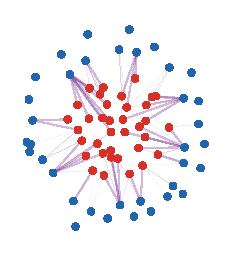
\includegraphics[width=.18\linewidth]{figures/dual-auction-progression/stage-0.pdf} &
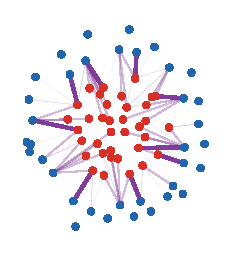
\includegraphics[width=.18\linewidth]{figures/dual-auction-progression/stage-1.pdf} &
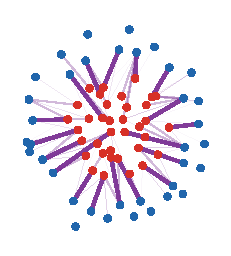
\includegraphics[width=.18\linewidth]{figures/dual-auction-progression/stage-2.pdf} &
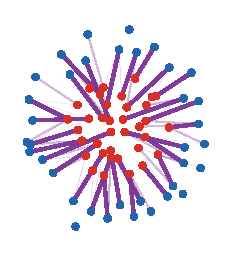
\includegraphics[width=.18\linewidth]{figures/dual-auction-progression/stage-3.pdf} &
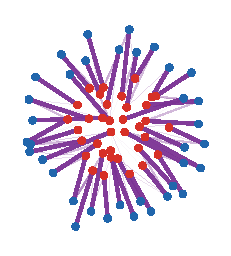
\includegraphics[width=.18\linewidth]{figures/dual-auction-progression/stage-4.pdf} \\[-.1em]
\small initial &
\small 2 bids &
\small 5 bids &
\small 7 bids &
\small final
\end{tabular}
\caption{\emph{Matrix view of actual auction iterates on the same diagonally dominant one-dimensional squared-distance assignment as Figure~\ref{fig:matching-hungarian-progression}.} Each panel records the current ownership state: unassigned bidders are shown as flat rows, while assigned bidders are shown as one-hot rows at their currently held target. The snapshots show initialization, intermediate price updates, and the final identity assignment satisfying complementary slackness.}
\index{complementary slackness}% strictindex
\label{fig:dual-auction-progression}
\end{figure}

\paragraph{Approximate optimality.}
The bidding invariant yields both finite termination and a quantitative suboptimality bound.

For fixed prices $p$, eliminating the bidder utilities $u_i$ in the dual minimization gives the convex objective
\[
	D(p)=\sum_j p_j+\sum_i \max_j(a_{i,j}-p_j),
\]
which comes from the dual constraints $u_i+p_j\geq a_{i,j}$. The auction update should thus be viewed as a price-adjustment method on this nonsmooth dual landscape, rather than as a generic gradient step: the proof of correctness is through approximate complementary slackness.
\index{complementary slackness}% strictindex

\begin{defn}[$\epsilon$-complementary slackness]\label{def-auction-eps-cs}
	An assignment $\sigma$ and prices $p$ satisfy $\epsilon$-complementary slackness if, for every source $i$,
	\[
		a_{i,\sigma(i)}-p_{\sigma(i)}
		\geq
		\max_j(a_{i,j}-p_j)-\epsilon.
	\]
	For a partial assignment, the same condition is required only for currently assigned sources.
\end{defn}

\begin{prop}[Auction invariant and finite termination]\label{prop-auction-termination}
\index{auction algorithm}% strictindex
	At every iteration of Algorithm~\ref{alg:auction-bidding}, each currently owned pair satisfies $\epsilon$-complementary slackness. Moreover, if
	\[
		\Delta_A\eqdef\max_{i,j}a_{i,j}-\min_{i,j}a_{i,j},
	\]
	then the algorithm terminates after at most
	\[
		1+\left\lfloor\frac{n(\Delta_A+\epsilon)}{\epsilon}\right\rfloor
	\]
	bids.
\end{prop}
\begin{proof}
	Immediately after source $i$ bids for $j_i$, its reduced profit there is
	\[
		a_{i,j_i}-p_{j_i}^{\mathrm{new}}=w_i-\epsilon,
	\]
	whereas every alternative has reduced profit at most $w_i$. Later bids only increase competing prices. The price of $j_i$ itself cannot change while $i$ remains its owner, because such a change would reassign $j_i$ and make $i$ unassigned. Thus every owned pair satisfies the claimed invariant.

	Each bid raises one price by at least $\epsilon$. After any nonterminal bid, at least one target different from the selected target remains unassigned; it has never been owned and still has price zero. Denote such a target by $k$. Since it was also available before the bid, the second-best value satisfies $w_i\geq a_{i,k}$, and hence
	\[
		p_{j_i}^{\mathrm{new}}=a_{i,j_i}-w_i+\epsilon
		\leq \Delta_A+\epsilon.
	\]
	Consequently, before the terminal bid the sum of all prices is at most $n(\Delta_A+\epsilon)$. Since this sum grows by at least $\epsilon$ per bid, there can be at most $n(\Delta_A+\epsilon)/\epsilon$ nonterminal bids, followed by at most one terminal bid.
\end{proof}

\begin{prop}[Auction optimality certificate]\label{prop-auction-eps-cs}
\index{optimality!certificate}% strictindex
	If a complete assignment $\sigma$ satisfies $\epsilon$-complementary slackness, then it is $n\epsilon$-optimal for the profit maximization problem, or equivalently $n\epsilon$-optimal for the original cost minimization problem. If all costs are integers and $\epsilon<1/n$, then $\sigma$ is optimal.
\index{complementary slackness}% strictindex
\end{prop}

\begin{proof}
	Let $\tau$ be any assignment. By $\epsilon$-complementary slackness,
	\[
		a_{i,\tau(i)}-p_{\tau(i)}
		\leq
		\max_j(a_{i,j}-p_j)
		\leq
		a_{i,\sigma(i)}-p_{\sigma(i)}+\epsilon.
	\]
	Summing over $i$ cancels prices, because both $\sigma$ and $\tau$ are permutations:
	\[
		\sum_i a_{i,\tau(i)}
		\leq
		\sum_i a_{i,\sigma(i)}+n\epsilon.
	\]
	Thus no assignment has profit more than $n\epsilon$ above that of $\sigma$. Since $a=-C$, the same statement says that the cost of $\sigma$ is at most $n\epsilon$ above the minimum cost. If the costs are integers, all assignment costs are integers; a gap strictly smaller than one therefore forces the gap to be zero.
\index{cost!assignment}% strictindex
\end{proof}

Propositions~\ref{prop-auction-termination} and~\ref{prop-auction-eps-cs} therefore give a complete correctness argument: the algorithm terminates with a complete assignment, and that assignment is $n\epsilon$-optimal. Sharper complexity bounds, $\epsilon$-scaling variants and efficient implementations are developed in~\cite{bertsekas1992auction,merigot2020optimaltransportalgorithms}.
\index{complementary slackness}% strictindex

\begin{rem}[$\epsilon$-scaling and relation with Sinkhorn]
\index{matrix!scaling}% strictindex
\index{Sinkhorn!algorithm}% strictindex
	In practice one starts with a coarse $\epsilon$ and repeatedly decreases it, warm-starting the prices and assignment. This $\epsilon$-scaling strategy is a homotopy method: large $\epsilon$ regularizes the combinatorial problem by enforcing a visible margin between the best and second-best reduced profits, while small $\epsilon$ recovers the exact dual certificate. If one wants a continuous-optimization analogy, the margin is closer to an exact-penalty or proximal continuation parameter than to a literal quadratic penalty.
\index{dual!certificate}% strictindex

	Sinkhorn scaling plays a parallel role for entropic OT. There, the hard minimum in the dual $c$-transform is replaced by a soft minimum, or log-sum-exp, with temperature $\epsilon$; in the auction algorithm, the hard maximum is kept but the complementary slackness condition is relaxed by $\epsilon$. Both methods therefore use an $\epsilon$-controlled dual continuation, and both recover the unregularized transport certificate as $\epsilon\to0$ under the usual assumptions. The outputs are different: Sinkhorn produces dense entropic couplings, whereas auction keeps a sparse assignment throughout.
\index{Sinkhorn!scaling}% strictindex
\index{entropic!OT}% strictindex
\index{log-sum-exp}% strictindex
\index{complementary slackness}% strictindex
\index{auction algorithm}% strictindex
\index{soft!minimum}% strictindex
\index{c-transform}% strictindex
\end{rem}

%%%%%%%%%%%%%%%%%%%%%%%%%%%%%%%%%%%%%%%%%%%%%%%%%%%%%%%%%%%%%%%%%%%%%%%%%%%
\section{General formulation}
\label{sec-dual-general}
\index{Kantorovich!duality}% strictindex
\index{continuous!dual}% strictindex

The continuous dual is the analytic counterpart of the discrete linear program. It uses continuous potentials because measures are probed through integration.

\paragraph{Continuous duality.}
The finite-dimensional price vectors become continuous test functions paired with the two marginals.

To extend this primal-dual construction to arbitrary measures, it is important to realize that measures are naturally paired in duality with continuous functions, using the pairing $\dotp{\f}{\al} \eqdef \int f \d \al$.
\index{measure-function duality}% strictindex

%  (a measure can only be accessed through integration against continuous functions). The duality is formalized in the following proposition, which boils down to Proposition~\ref{prop-duality-discr} when dealing with discrete measures.

\begin{prop}[Kantorovich duality]\label{prop-kantorovich-duality-general}
\index{Kantorovich!duality}% strictindex
	Assume that $\Xx$ and $\Yy$ are compact metric spaces and that $c\in\Cc(\Xx\times\Yy)$. Then
	\eql{\label{eq-dual-generic}
		\MK_\c(\al,\be) =
		\umax{(\f,\g) \in \Potentials(\c)}
			\int_\X \f(x) \d\al(x) + \int_\Y \g(y) \d\be(y),
	}
	where the set of admissible dual potentials is
\index{dual!potential}% strictindex
	\eql{\label{eq-dfn-pot-dual}
		\Potentials(\c) \eqdef \enscond{
			(\f,\g) \in \Cc(\X) \times \Cc(\Y)
		}{
			\forall (x,y), \f(x)+\g(y) \leq \c(x,y)
		}.
	}
	Here, $(\f,\g)$ is a pair of continuous functions, often called ``Kantorovich potentials''.
\index{Kantorovich!potential}% strictindex
	The same formula extends under the usual lower-semicontinuity and integrability assumptions, replacing maxima by suprema when dual optimizers need not exist.
\end{prop}
\begin{proof}
	Weak duality is immediate: if $f(x)+g(y)\leq c(x,y)$ and $\pi\in\Couplings(\al,\be)$, then
\index{duality!weak}% strictindex
	\[
		\int f\d\al+\int g\d\be
		=
		\int (f(x)+g(y))\d\pi(x,y)
		\leq
		\int c\d\pi.
	\]
	Taking the supremum over admissible potentials and the infimum over couplings gives the first inequality.
\index{admissible potential}% strictindex

	For the reverse inequality, write $V=\MK_\c(\al,\be)$ and consider the convex cone
\index{affine!map}% strictindex
\index{probability measure}% strictindex
\index{Radon measure}% strictindex
\index{topology!weak}% strictindex
	\[
		\mathcal K
		\eqdef
		\left\{\left(\pi_1,\pi_2,\int c\d\pi+r\right):
		\pi\in\Mm_+(\X\times\Y),\ r\geq0\right\}
	\]
	in $\Mm(\X)\times\Mm(\Y)\times\RR$, equipped with the weak topologies on the measure factors. This cone is closed. Indeed, convergence of the first marginal implies a uniform bound on the masses of the underlying nonnegative measures. Compactness of $\X\times\Y$ then gives a convergent subnet $\pi_k\rightharpoonup\pi$; continuity of marginalization and of $\pi\mapsto\int c\d\pi$ identifies the limit with an element of $\mathcal K$, while the limiting epigraph remainder remains nonnegative.

	For every $t<V$, the point $z_t=(\al,\be,t)$ does not belong to $\mathcal K$. Strong separation of this point from the closed convex cone gives a continuous linear functional. Because $\mathcal K$ is a cone containing the origin, the functional can be oriented so that, for some $F\in\Cc(\X)$, $G\in\Cc(\Y)$ and $\lambda\in\RR$,
	\[
		\int F\d\al+\int G\d\be+\lambda t<0
		\leq
		\int F\d\eta+\int G\d\zeta+\lambda s
		\qquad
		\text{for all }(\eta,\zeta,s)\in\mathcal K.
	\]
	Testing $(0,0,r)\in\mathcal K$ gives $\lambda\geq0$, while testing the element generated by $\pi=\de_{(x,y)}$ and $r=0$ gives
	$F(x)+G(y)+\lambda c(x,y)\geq0$. The multiplier cannot vanish: if $\lambda=0$, integrating this last inequality against $\al\otimes\be$ would contradict the strict inequality at $z_t$. Thus $\lambda>0$, and
	\[
		f\eqdef-F/\lambda,\qquad g\eqdef-G/\lambda
	\]
	satisfy $f\oplus g\leq c$ and
	$\int f\d\al+\int g\d\be>t$. Letting $t\uparrow V$ proves the reverse inequality.

	It remains to prove that the dual supremum is attained. Take a maximizing sequence $(f_k,g_k)$. Successively replace it by
	\[
		\widetilde g_k(y)=\min_x\{c(x,y)-f_k(x)\},
		\qquad
		\widetilde f_k(x)=\min_y\{c(x,y)-\widetilde g_k(y)\}.
	\]
	Each replacement preserves feasibility and cannot decrease the objective. Fixing $x_0\in\X$, use the gauge freedom
	$(\widetilde f_k,\widetilde g_k)\mapsto
	(\widetilde f_k-a_k,\widetilde g_k+a_k)$
	to impose $\widetilde f_k(x_0)=0$. Uniform continuity of $c$ shows that $\widetilde g_k$ inherits a common modulus in the second variable and $\widetilde f_k$ a common modulus in the first. The gauge gives a uniform bound on $\widetilde f_k$, and the first envelope then gives one on $\widetilde g_k$. Arzel\`a--Ascoli yields uniformly convergent subsequences. Their limit remains admissible and attains the dual supremum.
\end{proof}

\begin{rem}[Dual attainment from $c$-transforms]\label{rem-kantorovich-dual-attainment}
\index{dual!attainment}% strictindex
\index{c-transform}% strictindex
	The final part of the proof uses precisely the $c$-transforms introduced in Section~\ref{sec-c-transfo}. A continuous cost on a compact product has uniform moduli of continuity in both variables, and transformed potentials inherit those moduli by Proposition~\ref{prop-c-transform-lipschitz}. If the cost is Lipschitz, this specializes to a common Lipschitz bound; Lipschitz continuity is not required for attainment.
\index{Kantorovich!duality}% strictindex
\end{rem}

\paragraph{Complementary slackness.}
As in the finite problem, equality of primal and dual values localizes the support of every optimal coupling.

\begin{prop}[Continuous complementary slackness]\label{prop-continuous-complementary-slackness}
\index{complementary slackness}% strictindex
	For $\pi\in\Couplings(\al,\be)$ and $(f,g)\in\Potentials(\c)$,
	\[
		\int c\d\pi-\int f\d\al-\int g\d\be
		=
		\int\bigl(c(x,y)-f(x)-g(y)\bigr)\d\pi(x,y)
		\geq0.
	\]
	The coupling and potentials are respectively primal and dual optimal if and only if this gap vanishes. In that case,
	\eql{\label{eq-mk-pd-rel-cont}
		\Supp(\pi)
		\subset
		\enscond{(x,y)\in\X\times\Y}{f(x)+g(y)=c(x,y)}.
	}
\end{prop}
\begin{proof}
	The marginal identities give the equality, and admissibility gives nonnegativity. A zero gap is equivalent to equality of the feasible primal and dual values, hence to joint optimality by Proposition~\ref{prop-kantorovich-duality-general}. Finally, the slack is continuous and nonnegative. If it were positive at a point of $\Supp(\pi)$, it would be bounded below by a positive constant on a neighborhood of positive $\pi$-mass, contradicting its zero integral.
\end{proof}

The discrete case~\eqref{eq-dual} corresponds to the dual vectors being samples of the continuous potentials, namely $(\fD_i,\gD_j)=(\f(x_i),\g(y_j))$. Proposition~\ref{prop-continuous-complementary-slackness} is the exact analogue of Proposition~\ref{prop-discrete-complementary-slackness}.
\index{support}% strictindex
\index{optimal plan}% strictindex
For the one-dimensional quadratic cost, the continuous potentials can be read from the monotone map $T=F_\be^{-1}\circ F_\al$: on the active graph, $f'(x)=2(x-T(x))$ and $g=f^c$.
\index{quadratic!cost}% strictindex

\begin{figure}[ht]
\centering
\begin{tabular}{@{}ccc@{}}
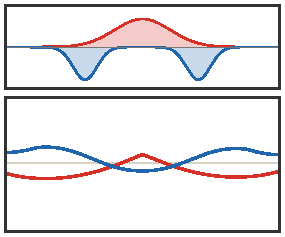
\includegraphics[width=.30\linewidth]{figures/dual-kantorovich-continuous-potentials/target-balanced.pdf} &
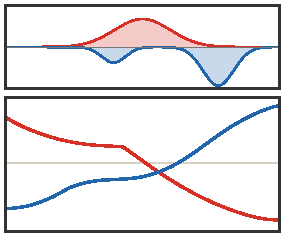
\includegraphics[width=.30\linewidth]{figures/dual-kantorovich-continuous-potentials/target-shifted.pdf} &
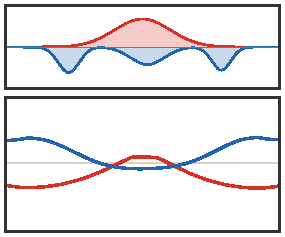
\includegraphics[width=.30\linewidth]{figures/dual-kantorovich-continuous-potentials/target-three-mode.pdf} \\[-.1em]
\small balanced target &
\small strongly shifted target &
\small three-mode target
\end{tabular}
\caption{\emph{Continuous Kantorovich potentials for the same source and target families as Figure~\ref{fig:dual-kantorovich-discrete-potentials}.} The upper strips show the source density $\al$ in red and the target density $\be$ in blue, including the strongly shifted and three-mode targets. The lower strips show potentials $f$ and $g=f^c$ for the quadratic cost $c(x,y)=|x-y|^2$, with the same gauge convention as in the discrete figure. The equality set $f(x)+g(y)=c(x,y)$ contains the monotone transport graph.}
\index{Kantorovich!potential}% strictindex
\index{quadratic!cost}% strictindex
\label{fig:dual-kantorovich-continuous-potentials}
\end{figure}

The same optimality condition is even more explicit if one plots the \emph{slack}
\[
	s(x,y) \eqdef c(x,y)-f(x)-g(y).
\]
Dual feasibility is the statement $s\geq0$, while complementary slackness says that an optimal coupling can only live where this slack vanishes. Figure~\ref{fig:dual-complementary-slackness-contacts} shows this zero set for increasingly structured one-dimensional transports, including a Gaussian source mapped to a three-component target mixture: the transported graph is not guessed from the potentials separately, but appears as the contact valley of the dual inequality.
\index{complementary slackness}% strictindex
\index{dual!slack}% strictindex

\begin{figure}[H]
\centering
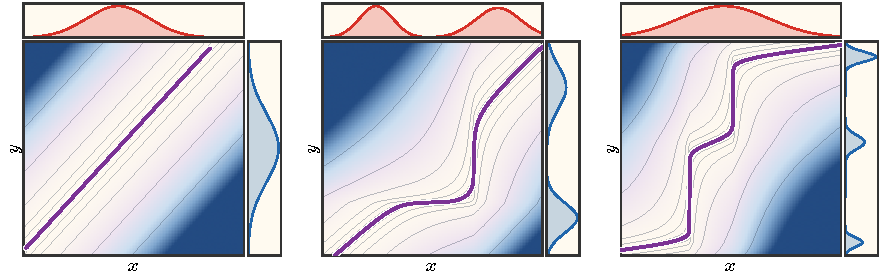
\includegraphics[width=.98\linewidth]{figures/dual-complementary-slackness-contacts/contacts.pdf}
\caption{\emph{Complementary slackness contacts for one-dimensional quadratic OT.} From left to right: transport between two Gaussian densities, transport between two-component Gaussian-mixture densities, and transport from one Gaussian density to a separated three-component mixture. Each central heatmap displays the nonnegative dual slack $s(x,y)=|x-y|^2-f(x)-g(y)$: pale colors mark the contact valley and darker blue means larger strict slack. The red top strip and blue side strip show the source and target densities. The violet curve is the quantile transport contact graph $(x,T(x))$, where $s(x,T(x))=0$ and the optimal Monge plan is supported.}
\index{complementary slackness}% strictindex
\index{dual!slack}% strictindex
\label{fig:dual-complementary-slackness-contacts}
\end{figure}

In contrast to the primal problem~\eqref{eq-mk-generic}, dual attainment is not immediate because $\Potentials(c)$ is neither compact nor controlled by a coercive objective. The $c$-transform resolves this issue: it selects canonical representatives that inherit the modulus of continuity of the cost, and a gauge condition then makes the family compact.
\index{c-transform}% strictindex


%%%%%%%%%%%%%%%%%%%%%%%%%%%%%%%%%%%%%%%%%%%%%%%%%%%%%%%%%%%%%%%%%%%%%%%%%%%
\section[c-transforms]{$c$-transforms}
\label{sec-c-transfo}

The $c$-transform is the operation that improves potentials without changing feasibility. It is both a proof device for dual attainment and the route from duality to Brenier's convex potentials.
\index{dual!attainment}% strictindex
\index{convex!potential}% strictindex

%%%%
\paragraph{Best-response potentials and the $c$-transform.}
\index{c-transform}% strictindex

Keeping a dual potential $\f$ fixed, one can maximize in closed form over the second potential in the dual problem~\eqref{eq-dual-generic}, which leads one to consider
\index{dual!potential}% strictindex
\index{dual!problem}% strictindex
\eq{
	\usup{\g \in \Cc(\Yy)} \enscond{
		\int g \d \be }{
			\foralls (x,y), \g(y) \leq c(x,y) - \f(x)
		}.
}
The constraint can be replaced by
\eq{
	\foralls y \in \Yy, \quad \g(y) \leq \f^\c(y)
}

\begin{defn}[$c$-transform]\label{def-c-transform}
\index{c-transform}% strictindex
	For a real-valued function $f:\Xx\to\RR$, its $c$-transform is the extended-real-valued function
	\eql{\label{eq-c-transform}
		\foralls y \in \Y, \quad
		\f^\c(y) \eqdef \uinf{x \in \X} \c(x,y) - \f(x).
	}
	For a real-valued function $g:\Yy\to\RR$, the $\bar c$-transform associated with $\bar c(y,x)=c(x,y)$ is
	\[
		\foralls x \in \X, \quad
		\g^{\bar\c}(x) \eqdef \uinf{y \in \Y} \c(x,y) - \g(y).
	\]
	When $\Xx,\Yy$ are compact, $c$ is continuous and the input potential is continuous, these infima are finite minima and the transformed potential is continuous.
\end{defn}
\begin{rem}[Discrete $c$-transform]\label{rem-discrete-c-transform}
\index{discrete!c-transform}% strictindex
\index{dual!potential}% strictindex
	If $\al=\sum_{i=1}^n a_i\de_{x_i}$ and $\be=\sum_{j=1}^m b_j\de_{y_j}$, the same definition applies to the finite spaces $\X=\{x_i\}_i$ and $\Y=\{y_j\}_j$. The dual potentials are then vectors $(\fD,\gD)\in\RR^n\times\RR^m$, as in Section~\ref{sec-discrete-dual}, and the cost is the matrix $\C\in\RR^{n\times m}$ with entries
	\[
		\C_{i,j}=c(x_i,y_j).
	\]
	With the present sign convention $f\oplus g\leq c$, the discrete transform of $\fD$ is the vector $\fD^\C\in\RR^m$ defined by
	\[
		(\fD^\C)_j
		=
		\min_{1\leq i\leq n} \C_{i,j}-\fD_i.
	\]
	This is a minimum because feasibility imposes the upper bound $\gD_j\leq \C_{i,j}-\fD_i$ for every $i$. Thus the largest feasible best response is the minimum of these upper bounds; formulas with a maximum correspond to a different sign convention, not to the dual constraint~\eqref{eq-dual}.
	With $\bar\C\eqdef\C^\top$, the opposite transform of $\gD$ is
	\[
		\gD^{\bar\C}\eqdef \gD^{\C^\top}\in\RR^n,
		\qquad
		(\gD^{\bar\C})_i
		=
		\min_{1\leq j\leq m} \C_{i,j}-\gD_j.
	\]
	Thus the continuous best-response operation reduces exactly to taking column minima for $\fD^\C$, or row minima for $\gD^{\bar\C}$, in shifted cost matrices. Chapter~\ref{sec-semidiscr-w1} studies the hybrid case where $\al$ has a density and $\be$ is discrete; then $g^{\bar c}(x)=\min_j c(x,y_j)-g_j$ is a lower envelope over target atoms, and the regions where each atom realizes the minimum are the Laguerre cells for the quadratic cost.
\index{Laguerre cell}% strictindex
\end{rem}
Since $\be$ is nonnegative, maximizing $\int \g \d \be$ saturates the bound $\g\leq\f^\c$ on $\Supp(\be)$, equivalently $\be$-almost everywhere.

\begin{figure}[H]
\centering
\begin{tabular}{@{}ccc@{}}
\small $p=1$ &
\small $p=2$ &
\small $p=4$ \\[-.15em]
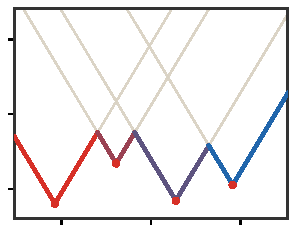
\includegraphics[width=.30\linewidth]{figures/dual-c-transform-envelope/p1.pdf} &
\index{c-transform}% strictindex
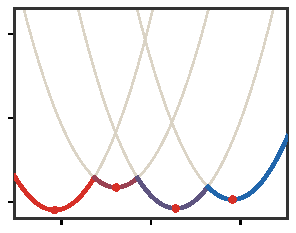
\includegraphics[width=.30\linewidth]{figures/dual-c-transform-envelope/p2.pdf} &
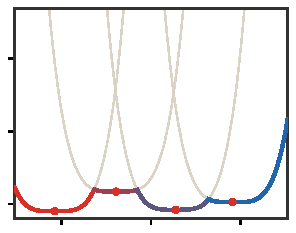
\includegraphics[width=.30\linewidth]{figures/dual-c-transform-envelope/p4.pdf}
\end{tabular}
\caption{\emph{Discrete $c$-transform as a lower envelope for costs $c_p(x,y)=|x-y|^p$.} The red circles are four source atoms $x_i$ with potential values $f_i$; the gray curves are the translated functions $y\mapsto c_p(x_i,y)-f_i$; the colored curve is their lower envelope $f^c(y)=\min_i c_p(x_i,y)-f_i$. This is the semi-discrete situation where $\X$ is finite, equivalently the source measure $\al$ is discrete; Chapter~\ref{sec-semidiscr-w1} studies the complementary case where the eliminated potential is supported on finitely many target atoms.}
\index{semi-discrete!OT}% strictindex
\label{fig:dual-c-transform-envelope}
\end{figure}

\begin{prop}[$c$-transforms solve the semi-relaxed problems]\label{prop-c-transform-semi-relaxed}
\index{c-transform}% strictindex
\index{semi-relaxed problem}% strictindex
	Assume the compactness and continuity hypotheses of Proposition~\ref{prop-kantorovich-duality-general}. For fixed $f\in\Cc(\X)$, the maximizers of the dual objective over all $g\in\Cc(\Y)$ such that $f\oplus g\leq c$ are exactly the functions satisfying $g=f^c$ $\be$-almost everywhere. Equivalently, $f^c$ gives the value of the one-marginal primal problem
	\[
		\inf_{\substack{\pi\in\Mm_+^1(\X\times\Y)\\ \pi_2=\be}}
		\int c(x,y)\d\pi(x,y)-\int f(x)\d\pi_1(x)
		=
		\int f^c(y)\d\be(y).
	\]
	Symmetrically, for fixed $g$, the maximizers over $f$ are the functions satisfying $f=g^{\bar c}$ $\al$-almost everywhere.
\end{prop}
\begin{proof}
	The constraint $f(x)+g(y)\leq c(x,y)$ for all $x$ is equivalent, for each fixed $y$, to
	\[
		g(y)\leq \inf_x c(x,y)-f(x)=f^c(y).
	\]
	Since $\be$ is nonnegative, the largest possible value of $\int g\d\be$ is obtained by saturating this pointwise upper bound on the support of $\be$. The proof for $f=g^{\bar c}$ is identical after exchanging the two marginals.

	For the primal formula, disintegrate any feasible $\pi$ as $\pi(\d x,\d y)=\pi_y(\d x)\be(\d y)$. Then
\index{disintegration}% strictindex
	\[
		\int c\d\pi-\int f\d\pi_1
		=
		\int\left(\int (c(x,y)-f(x))\d\pi_y(x)\right)\d\be(y)
		\geq
		\int f^c(y)\d\be(y).
	\]
	The argmin of $x\mapsto c(x,y)-f(x)$ is nonempty and compact. The measurable maximum theorem provides a Borel selector $x_\star(y)$ from these argmins. The coupling
	$\pi(\d x,\d y)=\de_{x_\star(y)}(\d x)\be(\d y)$
	then attains equality.
\index{measurable selection}% strictindex
\end{proof}

The improvement must be performed sequentially. Starting from an admissible pair, first update
\[
	(f,g)\longmapsto(f,f^c),
\]
and then update
\[
	(f,f^c)\longmapsto(f^{c\bar c},f^c).
\]
Each step preserves feasibility and cannot decrease the dual objective. By contrast, simultaneously replacing an arbitrary pair by $(g^{\bar c},f^c)$ need not preserve feasibility, because the two best responses were computed against different old coordinates. For example, if $c\equiv0$ and $f=g\equiv-1$, the original pair is feasible, but both transforms equal $1$, so the simultaneous update is not. Functions of the form $f^c$ and $g^{\bar c}$ are called $c$-concave and $\bar c$-concave, respectively. These transforms also give canonical extensions of dual solutions beyond the active supports.
\index{dual!potential}% strictindex
\index{c-transform}% strictindex

\begin{prop}[Modulus stability of $c$-transforms]\label{prop-c-transform-lipschitz}
\index{Lipschitz!stability}% strictindex
\index{modulus of continuity}% strictindex
	Suppose that $\omega_\Y$ is a modulus such that
	\[
		|c(x,y)-c(x,y')|
		\leq\omega_\Y\bigl(d_\Y(y,y')\bigr)
		\qquad\text{for all }x,y,y'.
	\]
	Then every finite $f^c$ has the same modulus. Symmetrically, a uniform modulus $\omega_\X$ of $c$ in its first variable is inherited by $g^{\bar c}$. In particular, a uniform $L$-Lipschitz bound on the cost yields an $L$-Lipschitz bound on the corresponding transform.
\end{prop}
\begin{proof}
	For each $x$, set $F_x(y)=c(x,y)-f(x)$ and $F(y)=f^c(y)=\inf_x F_x(y)$. Since all the functions $F_x$ share the modulus $\omega_\Y$,
	\[
		|F(y)-F(y')|
		=
		\left|\inf_x F_x(y)-\inf_x F_x(y')\right|
		\leq
		\sup_x |F_x(y)-F_x(y')|
		\leq
		\omega_\Y\bigl(d_\Y(y,y')\bigr).
	\]
	The proof in the first variable is identical.
\end{proof}

This stability is crucial for dual attainment. On compact spaces, continuity of $c$ already supplies uniform moduli; after sequential closure and a harmless additive gauge, compactness follows from the Arzel\`a--Ascoli theorem.
\index{dual!attainment}% strictindex
\index{admissible potential}% strictindex

\paragraph{Euclidean case.}

The Euclidean quadratic cost is the model case where $c$-transforms become ordinary convex conjugates after removing the quadratic terms. This is the algebraic bridge between Kantorovich duality and Brenier maps.
\index{Kantorovich!duality}% strictindex
\index{convex!conjugate}% strictindex
\index{quadratic!cost}% strictindex
\index{Brenier!map}% strictindex
\index{c-transform}% strictindex

It is convenient to normalize the quadratic cost as
$q(x,y)=\frac12\norm{x-y}^2$. For any $\pi\in\Couplings(\al,\be)$,
\[
	\int q(x,y)\d\pi(x,y)
	=
	\frac12\int\norm{x}^2\d\al(x)
	+\frac12\int\norm{y}^2\d\be(y)
	-\int \dotp{x}{y}\d\pi(x,y).
\]
The first two terms depend only on the marginals, so quadratic transport reduces to the bilinear cost $c(x,y)=-\dotp{x}{y}$. For this cost,
\[
	f^c(y)
	=
	\inf_x -\dotp{x}{y}-f(x)
	=
	-(-f)^*(y),
	\qquad
	h^*(y)\eqdef\sup_x \dotp{x}{y}-h(x).
\]
On the full Euclidean space, $f^{c\bar c}=-(-f)^{**}$; hence $c$-closed functions are negatives of lower semicontinuous convex functions, and the closure is the smallest upper semicontinuous concave majorant of $f$. On restricted compact domains, the same statement holds with the additional restriction that the supporting slopes belong to the opposite domain. Thus it coincides with the ordinary concave envelope only when that slope restriction is inactive.
\index{convex!function}% strictindex
\index{c-transform}% strictindex

\begin{rem}[Proof of Brenier's theorem]\label{rem-proof-brenier}
\index{Brenier!theorem}% strictindex
	Let $\al,\be\in\Pp_2(\RR^d)$ and assume that $\al$ has a density. For $q(x,y)=\frac12\norm{x-y}^2$, let $(u,v)$ be a closed optimal dual pair and set
	\[
		\phi(x)\eqdef\frac12\norm{x}^2-u(x),
		\qquad
		\psi(y)\eqdef\frac12\norm{y}^2-v(y).
	\]
	The constraint $u(x)+v(y)\leq q(x,y)$ becomes
	$\phi(x)+\psi(y)\geq\dotp{x}{y}$. Since the pair is closed,
	\[
		v(y)=\inf_x\{q(x,y)-u(x)\},
		\qquad
		u(x)=\inf_y\{q(x,y)-v(y)\}.
	\]
	The preceding conjugacy calculation gives $\psi=\phi^*$ and $\phi=\psi^*$, so $\phi$ is convex. Complementary slackness then shows that an optimal plan satisfies
\index{optimal plan}% strictindex
		\[
			\Supp(\pi)
			\subset
			\enscond{(x,y)}{\phi(x)+\phi^*(y)=\dotp{x}{y}}.
		\]
	By the Fenchel equality criterion, the contact condition is equivalent to $y\in\partial\phi(x)$. Convex functions are differentiable Lebesgue-almost everywhere, hence $\al$-almost everywhere, so $\partial\phi(x)$ is a singleton for $\al$-almost every $x$. This yields the Brenier map $T=\nabla\phi$ and explains why the optimal coupling is concentrated on a graph. Multiplying the cost by two rescales the dual potentials but leaves this map unchanged, recovering the convention $c(x,y)=\norm{x-y}^2$ used elsewhere in the book.
\index{optimal coupling}% strictindex
\index{convex!function}% strictindex
\index{Brenier!map}% strictindex
\end{rem}


%%%%
\paragraph{Why hard alternating optimization stops.}
\index{alternating!optimization}% strictindex

A crucial property of the Legendre transform is that $f^{***}=f^*$, while $f^{**}$ is the lower-semicontinuous convex envelope of a proper function $f$. Analogous identities explain why exact alternating $c$-transform updates stop after one full cycle. The required convex-analytic background is standard in Rockafellar's theory~\cite{rockafellar2015convex}.
\index{convex!envelope}% strictindex
\index{convex!function}% strictindex
\index{Legendre transform}% strictindex
\index{c-transform}% strictindex

\begin{prop}[Algebra of $c$-transforms]\label{prop-c-transform-algebra}
Writing $\f^{c\bar c}\eqdef(\f^c)^{\bar c}$, the following pointwise identities hold whenever the transforms are well defined:
	\[
		\textnormal{(i) } f \leq f' \Rightarrow f^{c}\geq f'^{c},
		\qquad
		\textnormal{(ii) } f^{\c\bar{\c}} \geq f,
		\qquad
		\textnormal{(iii) } g^{\bar{\c}\c} \geq g,
		\qquad
		\textnormal{(iv) } \f^{\c\bar{\c}\c}=\f^{\c}.
	\]
\end{prop}

\begin{proof}
	The order reversal in (i) follows directly from the minus sign in the definition. For every $x$ and $y$,
	\[
		f^c(y)=\inf_{x'}\{c(x',y)-f(x')\}
		\leq c(x,y)-f(x),
	\]
	so $c(x,y)-f^c(y)\geq f(x)$. Taking the infimum over $y$ proves (ii), and exchanging the two spaces proves (iii). Finally, (ii) and the order reversal imply
	$f^c\geq f^{c\bar c c}$, whereas (iii) applied to $g=f^c$ gives
	$f^{c\bar c c}\geq f^c$. This proves (iv).
\end{proof}

This invariance shows that exact block maximization reaches a coordinatewise fixed point after one full cycle. Starting from any source potential $f$, the sequential updates are
\index{dual!potential}% strictindex
\eql{\label{eq-iter-c-trans}
	(f,g) \mapsto (f,f^c) \mapsto (f^{c\bar c},f^c) \mapsto (f^{c\bar c},f^{c\bar c c}) =  (f^{c\bar c},f^c) \ldots
}
The resulting pair is dual feasible, but it need not maximize the joint dual objective because its value still depends on the arbitrary initialization $f$.
\index{stationarity}% strictindex

\begin{alg}[Hard alternating $c$-transform closure]\label{alg:hard-c-transform-closure}
\index{c-transform}% strictindex
\textbf{Input:} Source potential $f$ on $\X$, cost $c$.

\textbf{Output:} A $c$-closed admissible pair $(\tilde f,\tilde g)$.

\textbf{Set} target best response:
\(g=f^c, \qquad g(y)=\inf_{x\in\X}\{c(x,y)-f(x)\}.\)

\textbf{Set} source closure:
\(\tilde f=g^{\bar c}=f^{c\bar c}.\)

\textbf{Set} closed target potential:
\(\tilde g=\tilde f^c=f^{c\bar c c}=f^c.\)
\par
\textbf{Return} $(\tilde f,\tilde g)=(f^{c\bar c},f^c)$.
\end{alg}

The issue is therefore not that the best responses are inaccurate, but that hard closure becomes idempotent before solving the joint optimization problem. Entropic regularization changes these hard minima into soft log-sum-exp responses. Their alternating updates are no longer exhausted by one closure cycle and lead to the Sinkhorn scaling algorithm studied in Chapter~\ref{sec-sinkhorn}.
\index{Sinkhorn!algorithm}% strictindex
\index{entropic!regularization}% strictindex

For the bilinear cost $c(x,y)=-xy$ on a compact interval, $f^{c\bar c}$ is the smallest concave majorant representable with slopes in the opposite interval. In Figure~\ref{fig:dual-alternating-c-transform-failure}, the displayed interval contains all relevant supporting slopes, so this restricted closure agrees with the ordinary concave envelope. A hard transform removes non-concave oscillations in one step rather than producing a gradual ascent.

\begin{figure}[ht]
\centering
\begin{tabular}{@{}cc@{}}
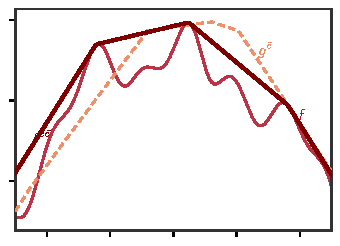
\includegraphics[width=.46\linewidth]{figures/dual-alternating-c-transform-failure/source-concave-closure.pdf} &
\index{c-transform}% strictindex
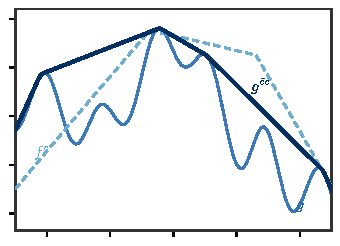
\includegraphics[width=.46\linewidth]{figures/dual-alternating-c-transform-failure/target-concave-closure.pdf} \\[-.1em]
\small source-side closure & \small target-side closure
\end{tabular}
\caption{\emph{Hard $c$-transforms for the bilinear cost $c(x,y)=-xy$.} The source-side panel uses a reddish palette and starts from a sharply oscillatory potential $f$; the target-side panel uses a blueish palette and starts from a visually different potential $g$. Dark curves are the double-transform closures $f^{c\bar c}$ and $g^{\bar c c}$, while dashed lighter curves are the one-sided best responses $g^{\bar c}$ and $f^c$ after a harmless vertical gauge shift. The plotted domains contain the relevant supporting slopes, so the restricted closures coincide here with ordinary concave majorants. The figure illustrates why exact alternating best responses are useful for dual certificates but do not give the smooth iterative dynamics later provided by entropic regularization.}
\index{entropic!regularization}% strictindex
\index{dual!certificate}% strictindex
\label{fig:dual-alternating-c-transform-failure}
\end{figure}
